\chapter{Interpretando a extensão STS e comparando-a com a MQ}
\label{chap:cap3}

Neste capítulo, vamos explorar algumas consequências da extensão STS, fornecendo uma interpretação mais precisa das soluções de sua equação ''dinâmica'', Eq.~(\ref{SchroT}), e comparando as informações contidas em $|\psi(t)\rangle $ e $|\pmb{\phi}(x)\rangle$. Uma interpretação dos autoestados de observáveis na extensão STS também será discutida. Ressaltamos que a partir de agora os resultados apresentados são originais desta dissertação.



\section{$|\psi(t)\rangle$ na base de energia {\textit versus} $|\pmb{\phi}(x)\rangle$ na base de momento}
\label{sec:bases}

A equação de autovalor de energia na MQ usual é equivalente à equação de autovalor de momento na extensão STS. Assim, conforme investigaremos, um potencial dependente do tempo na equação de Schrödinger~(\ref{Schro}) tem um efeito análogo a um potencial dependente do espaço na equação de Schrödinger EC~(\ref{SchroT}). Dito isso, consideramos $V=V(x,t)$ para lidarmos com o caso mais geral possível. Nesta seção iremos comparar as soluções gerais $|\psi(t)\rangle$ e $|\pmb{\phi}(x)\rangle$ nas bases de energia e momento, respectivamente. Vamos começar revisando a MQ usual para um hamiltoniano dependente do tempo~\cite{sakurai}. Primeiro, os autoestados de energia intantâneos satisfazem
\begin{equation}\label{SchroE1}
{\hat {\textrm H}}(t)|E_a(t)\rangle = E_a(t)|E_a(t)\rangle,
\end{equation}
onde $a$ é uma variável contínua tal que $\langle E_{a'}(t)|E_a(t)\rangle=\delta(a'-a)$ e $\int da |E_a(t)\rangle {\langle} E_a(t)|=1$. Semelhante à $|\psi(t)\rangle$, estamos omitindo o índice $t$ em $|E_a(t)\rangle$.


Um estado arbitrário em ${\mathcal H}_t$ pode então ser expandido nesta base instantânea de energia,
\begin{equation}\label{expansion}
    \ket{\psi(t)}=\int da ~ {\bar \psi}(E_a|t) \ket{E_a(t)},
\end{equation}
onde
\begin{equation}\label{PsiE}
    {\bar \psi}(E_a|t) \equiv {\langle} E_a(t)|\psi(t)\rangle= C(a|t)e^{i \theta_a(t)},
\end{equation}
com $\theta_a(t)=-1/\hbar\int_0^t \dd{t'}E_a(t')$ sendo a fase dinâmica. Da equação de Schrödinger~(\ref{Schro}), é fácil ver que o coeficiente $C(a|t)$ satisfaz
\begin{equation}\label{Ca}
    \frac{dC(a|t)}{dt}=-\int \dd{a'} C(a'|t)e^{i\Delta \theta_{a'a}(t)}\bra{E_a(t)}\frac{d}{dt}\ket{E_{a'}(t)},
\end{equation}
onde introduzimos $\Delta \theta_{a'a}(t)=\theta_{a'}(t)- \theta_a (t)$. Observe que ${\mathcal P}(E_{a}|t)=|{\bar \psi}(E_{a}|t)|^2=|C(a|t)|^2$ ($\theta_{a}(t)$ é um número real) é a densidade de probabilidade de medir a partícula com energia $E_{a}$, dado que a medição ocorre no tempo $t$. Agora, projetando a Eq.~(\ref{expansion}) em $|x\rangle_t$ produz
\begin{equation}\label{SolX3}
\psi(x|t)={_t\langle} x|\psi(t)\rangle=\int da ~\bar{\psi} (E_a|t)  \psi_a(x|t),
\end{equation}
onde $\psi_a(x|t)={_t\langle} x|E_a(t)\rangle_t$ é a amplitude de probabilidade da partícula ser encontrada na posição $x$, dado que sua energia é $E_a$ e o observação acontece no tempo $t$. Note que o índice $a$ representa uma variável condicional de modo que $\psi(x|E_a,t)$ também seria uma notação conveniente para ${_t\langle} x|E_a(t)\rangle_t$.

Para o hamiltoniano~(\ref{ruleX}), a projeção da Eq.~(\ref{SchroE1}) em $ \ket{x}$ resulta em
\begin{equation}\label{SchroXE}
    \left[-\frac{\hbar^2}{2m}\pdv[2]{x}+V(x,t) \right]\psi_a(x|t)=E_a(t) ~\psi_a(x|t).
\end{equation}
Em particular, para a situação de partícula livre, onde $[{\hat{H}},\hat{P}]=0$, $\psi_a(x|t)={_t\langle} x|E_a(t) \rangle$ torna-se independente do tempo e é dado por
\begin{eqnarray}\label{SolXFree}
\psi_E^\pm(x)=\sqrt{\frac{m}{2\pi \hbar }}\frac{1}{(2E)^{1/2}}\exp{\pm \frac{ i\sqrt{2mE}x}{\hbar}},
\end{eqnarray}
onde $\pm$ refere-se ao sinal do momento. Além disso, ${\bar \psi}(E_a|t)$ da Eq.~(\ref{PsiE}) pode ser escrito como ${\bar \psi}^{\pm}(E|t)={\bar \psi}^{\pm}(E) e^{-iEt/\hbar}$ e a solução geral~(\ref{SolX3}) torna-se
\begin{equation}\label{SolXL}
    \psi(x|t)=\int_{0}^{\infty} dE ~ \big[{\bar \psi}^+(E) \psi_E^+(x)+{\bar \psi}^-(E)  \psi_E^-(x)\big]e^{-iEt/\hbar},
\end{equation}
com ${\mathcal P}^{\pm}(E|t)=|{\bar \psi}^{\pm}(E)|^2$ independente do tempo.








A análise equivalente na extensão STS começa com a equação de autoestado do momento,
\begin{equation}\label{SchroTP1}
\hat{\mathbb P}(x) \ket{\pmb{P}_b(x)}= P_b(x)|\pmb{P}_b(x)\rangle
\end{equation}
[analogamente à Eq.~(\ref{SchroE1})], onde
\begin{equation}\label{Pb}
\ket{\pmb{P}_b(x)}=\mqty(|P^+_b(x)\rangle   \\ |P^-_b(x)\rangle)
\end{equation}
e, novamente, $b$ é uma variável contínua onde, ${\langle} \pmb{P}_{b'}(x)|\pmb{P}_b(x)\rangle=\delta(b'-b)$ e $\int db |\pmb{P}_b(x)\rangle{\langle} \pmb{P}_b(x)|=1$. Aqui também estamos omitindo o índice $x$ nos autoestados de momento. Observe que, assim como os potenciais dependentes do tempo na MQ usual produzem auto-estados de energia dependentes do tempo, um potencial dependente do espaço na extensão STS leva a auto-estados de momento dependentes do espaço. Isso significa que os estados com momento bem definido dependem da posição em que descrevemos a partícula. Em contraste, lembre-se que as autofunções de momento (energia) na MQ usual (extensão STS) são sempre as mesmas, proporcionais a $\exp{iPx/\hbar}$ ($\exp{-iEt/\hbar}$).


Analogamente à Eq.~(\ref{expansion}), utilizando da linearidade da equação de Shrödinger EC, um estado físico arbitrário em ${\mathcal{H}}_x$ na posição $x$ pode então ser expandido na base de momento como
\begin{equation}\label{expansionT}
    \ket{{\pmb \phi}(x)}=\int db~ {\tilde \phi}(P_b|x) \ket{{\pmb P}_b(x)},
\end{equation}
onde
\begin{equation}\label{phiP}
   {\tilde \phi}(P_b|x)\equiv \langle \pmb{P}_b(x)|\pmb{\phi}(x)\rangle= C(b|x)e^{i\theta_b(x)},
\end{equation}
com $\theta_b(x)=1/\hbar\int_0^x d x^\prime P_b(x')$ sendo o equivalente à fase dinâmica $\theta_a(t)$ na MQ usual. A partir da equação de Schrödinger EC~(\ref{SchroT}), pode-se verificar facilmente que o coeficiente $C_b(x)$ satisfaz uma equação semelhante à~(\ref{Ca}),
\begin{equation}
    \frac{dC(b|x)}{dx}=-\int d{b'} C(b'|x)e^{i\Delta \theta_{b'b}(t)}\bra{\pmb{P}_b(x)}\frac{d}{dx}\ket{\pmb{P}_{b'}(x)},
\end{equation}
onde $\Delta \theta_{b'b}(x)=\theta_b'(x)-\theta_b(x)$. Agora, nós temos
\begin{equation}\label{prob}
{\mathcal P}(P_b|x)=\frac{|{\tilde \phi}(P_b|x)|^2}{{\langle \pmb{\phi}(x)|\pmb{\phi}(x) \rangle}}
\end{equation}
como a amplitude de probabilidade de medir o estado com momento $P_b$, dado que a medição ocorre na posição $x$. Observe que $e^{i \theta_b(x)}$ é relevante para a Eq.~(\ref{prob}), pois $\theta_b(t)$ pode ser um número puramente imaginário. Projetando a Eq.~(\ref{expansionT}) em $|t\rangle_x$, obtemos uma expansão análoga à Eq.~(\ref{SolX3}) para a extensão STS,
\begin{equation}\label{SolT3}
{\pmb \phi}(t|x)={_x\langle} t|\phi(t)\rangle=\int db ~{\tilde \phi}(P_b|x) {\pmb \phi}_b(t|x),
\end{equation}
onde  
\begin{equation}\label{phib}
   \pmb{\phi}_b(t|x)=\mqty({_x\langle} t|P^+_b(x)\rangle   \\ {_x\langle}t|P^-_b(x)\rangle)\equiv \mqty( \phi^+_b(t|x)   \\ \phi^-_b(t|x) )
\end{equation}
é a amplitude de probabilidade da partícula chegar no tempo $t$, dado que seu momento é $P_b(x)$ e o detector está na posição $x$. 


Agora, usando $\mathbbm P$ definido na Eq.~(\ref{ruleP}), a projeção da Eq.~(\ref{SchroTP1}) em $|t\rangle_x$ resulta em
\begin{equation}\label{SchroTP}
\sigma_z \sqrt{2m\left(i\hbar \pdv{t}-V(x,t)\right)}\pmb{\phi}_b(t|x)=P_b(x)\pmb{\phi}_b(t|x).
\end{equation}
A Ref.~\cite{Dias} analisou a equação de autovalor do momento para a situação de partícula livre, onde $[{\hat {\mathbb P}},\hat {\mathbb H}]=0$. Em nossa situação, análogo à Eq.~(\ref{SolXFree}) na MQ usual, $\pmb{\phi}_b(t|x)$ definido na Eq.~(\ref{phib}) torna-se independente do espaço, e aqui é dado por duas funções vetoriais independentes,
A Ref.~\cite{Dias} analisou a equação de autovalor do momento para a situação de partícula livre, onde $[{\hat {\mathbb P}},\hat {\mathbb H}]=0$. Nossa situação, análogo às Eqs.~(\ref{SolXFree}) na MQ usual, $\pmb{\phi}_b(t|x)$ definido na Eq.~(\ref{phib}) torna-se independente do espaço, e aqui é dado por duas funções vetoriais independentes,
\begin{equation}\label{SolTL}
    \pmb{\phi}_{P_+}(t|x)=\mqty(\phi^+_{P_+}(t|x)   \\  0)
\end{equation}
e
\begin{equation}\label{SolTL}
   \pmb{\phi}_{P_-}(t|x)=\mqty(0  \\  \phi^-_{P_-}(t|x) ),
\end{equation}
com
\begin{eqnarray}\label{SolTFree}
\phi^{\pm}_{P_{\pm}}(t|x)=\phi^{\pm}_{P_{\pm}}(t)=\sqrt{\frac{|P_\pm|}{2\pi
m\hbar}}~\exp{-\frac{i(P_\pm)^2t}{2m\hbar}}.
\end{eqnarray}
e $P_\pm=\pm \sqrt{2mE}$, onde $E$ é a energia da partícula. Além disso, ${\tilde \phi}(P_b|x)$ definido na Eq.~(\ref{phiP}) pode ser escrito como
\begin{eqnarray}\label{phiPFree}
  {\tilde \phi}(P_{\pm}|x)={\tilde \phi}(P_\pm)e^{ iP_{\pm}x/\hbar},
\end{eqnarray} 
Considerando $E>0$ e definindo $\tilde{\phi}^{\pm}(P) \equiv \tilde{\phi} (P_{\pm})$, com $P=|P_\pm|$, a solução geral~(\ref{SolT3}) torna-se
\begin{eqnarray}\label{SolTL}
    \pmb{\phi}(t|x) = \int_0^\infty dP\big[{\tilde \phi}^+(P)\pmb{\phi}_{P_+}(t) e^{iPx/\hbar} + {\tilde \phi}^-(P)  \pmb{\phi}_{P_-}(t)e^{-iPx/\hbar} \big],
\end{eqnarray}
onde seu módulo quadrado normalizado é $\rho(t|x)$ dado na Eq.~(\ref{pd}). Vale a pena notar a semelhança entre as Eqs.~(\ref{SchroXE})-(\ref{SolXL}) e as Eqs.~(\ref{SchroTP})-(\ref{SolTL}). Diferente da MQ usual, onde ${\mathcal P}(E|t)=|{\bar \psi}(E)|^2$ é independente do tempo para partículas livres, ${\mathcal P}(P_{ \pm}|x)=|{\tilde \phi}^{\pm}(P)|^2/\langle \pmb{\phi}(x)|\pmb{\phi}(x)\rangle$ [ver Eq.~(\ref {prob})] pode depender de $x$ devido ao fator de normalização $\langle \pmb{\phi}(x)|\pmb{\phi}(x)\rangle$. Exploraremos essa diferença mais profundamente na próxima seção. 



\section{Uma interpretação mais precisa do formalismo STS e sua conexão com a MQ}
\label{sec:interpretando}

Vamos iniciar essa seção lembrando que os modelos existentes para o TOA ideal assumem que sua distribuição temporal é uma propriedade que depende apenas do estado quântico da partícula, $|\psi(t)\rangle$. Assim, se a extensão STS é uma teoria correta, devemos saber se é possível obter $|\pmb{\phi}(x)\rangle$ (que também visa prever TOA's ideais) apenas usando $|\psi(t )\rangle$ ou se $|\pmb{\phi}(x)\rangle$ contém informações sobre o sistema complementar à MQ.

Comecemos com a diferença física entre as notações $|\rangle_t$ e $|\rangle_x$. Quando se diz, por exemplo, que um sistema tem momento bem definido na MQ, implicitamente, está-se afirmando que $|\psi(t)\rangle=|P\rangle_t$, ou seja, a partícula tem momento $P$ no instante de tempo $t$. Portanto, autoestados na MQ referem-se à uma propriedade bem definida em um tempo fixo, justificando a notação $|\rangle_t$. Por outro lado, na extensão STS, $\left|\phi^{+}(x)\right\rangle=|P\rangle_x$ significa que a partícula tem momento $P$ na posição $x$, ou seja, a partícula chega em $x$ com momento $P$.


Para dar uma interpretação da solução da equação de Schrödinger EC~(\ref{SchroT}), primeiramente, precisamos ter em mente a informação que a equação de Schrödinger dependente do tempo fornece: Considerando uma função de onda inicial $ \psi(x|t_0)$ --- a amplitude de probabilidade de encontrar a partícula na posição $x$, dado que a observação ocorre no tempo inicial $t_0$ --- a solução da equação de Schrödinger, $\psi(x|t)$, é a amplitude de probabilidade de encontrar a partícula em $x$, dado que agora a observação ocorre em um momento posterior $t>t_0$. Observe que o tempo é um parâmetro clássico externo (o hora do relógio do laboratório) e, portanto, pode ser escolhido com precisão arbitrária para avaliar o estado do sistema e suas probabilidades.


Conforme discutido na seção anterior, a extensão STS é formulada trocando os papéis de posição e tempo (e energia e momento) na MQ. Portanto, seguindo o mesmo raciocínio do parágrafo anterior sobre as soluções da equação de Schrödinger, e tomando $x \rightleftarrows t$, a interpretação das soluções da equação de Schrödinger EC~(\ref{Schro2T}) torna-se a seguinte: Considerando uma função de onda EC ``inicial'' $\pmb{\phi}(t|x_0)$ --- a amplitude de probabilidade da partícula chegar no instante $t$, dado que a posição ``inicial'' do detector é $x_0$ --- a solução da Eq.~(\ref{Schro2T}), $\pmb{\phi}(t| x)$, é a amplitude de probabilidade da partícula chegar no instante $t$, dado que se move o detector para uma nova posição $x$. Para entender melhor esta interpretação, na Fig.~\ref{fig:timevsspace}, ilustramos a diferença entre a evolução temporal da MQ e a ``evolução espacial'' da sua extensão STS. Perceba que a condição ``inicial'' na extensão STS é na verdade uma condição de contorno para $\pmb{\phi}(t|x)$.

\begin{figure}[H]
    \centering
    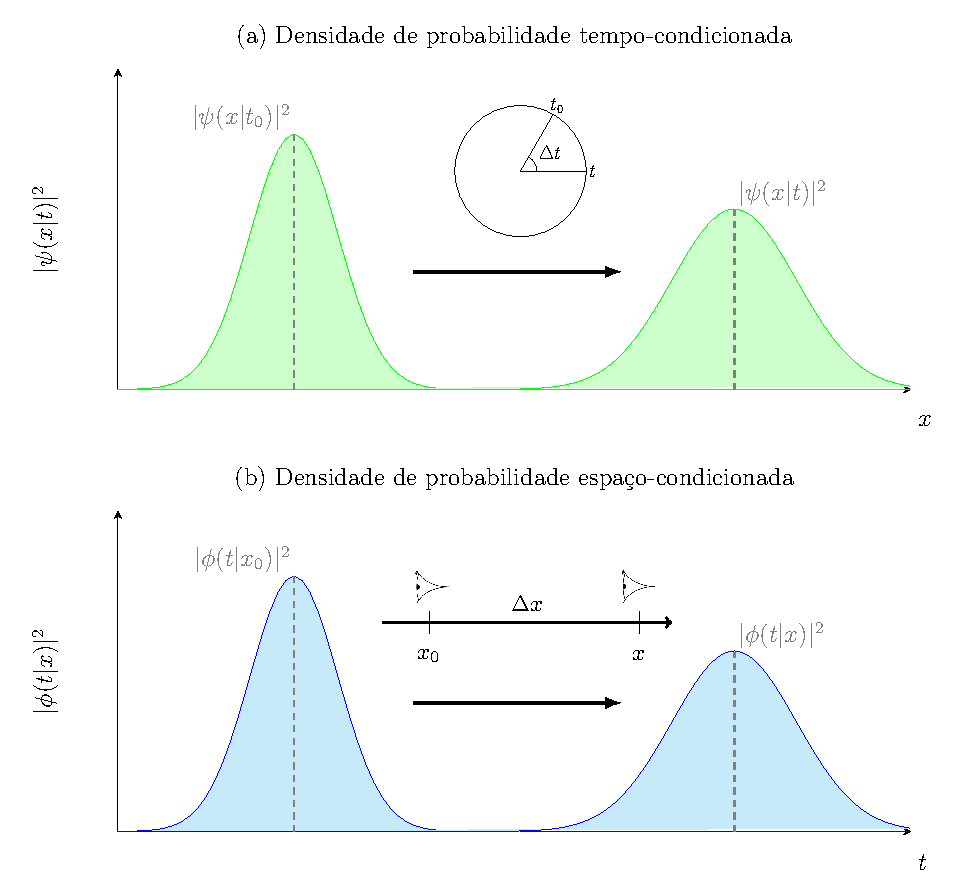
\includegraphics[width=15cm]{anexos/final_sketch_pt.pdf}
    \caption{Os dois sistemas descrevem diferentes situações físicas e têm diferentes propósitos experimentais; enquanto a densidade de probabilidade da mecânica quântica de Schrödinger (a) representada por $|\psi(x|t)|^2$ descreve uma situação em que medimos a posição de uma partícula dado um instante de tempo $t$, na teoria STS (b) representado por $|\pmb{\phi}(t|x)|^2$ medimos o tempo de chegada de uma partícula dada uma posição $x$ no espaço.}
    \label{fig:timevsspace}
\end{figure}


À primeira vista, pode-se pensar que a extensão STS não é projetada para responder ao problema tradicional TOA: Dada uma partícula com uma função de onda de momentos positivos em $t_0$, $\psi(x|t_0)$, restrita à uma região $x<x^* $, quando essa partícula chega na posição $x^*$? Seguindo a interpretação acima, assim como a equação de Schrödinger fornece translações temporais de uma função de onda previamente conhecida $\psi(x|t_0)$, a equação de Schrödinger EC~(\ref{Schro2T}) descreve translações espaciais de uma função de onda EC $\pmb{\phi}(t|x_0)$ que também deve ser conhecida. No entanto, se $\psi(x|t)$ e $\pmb{\phi}(t|x)$ compartilham informações comuns sobre outros observáveis, por exemplo, energia e/ou momento, $\psi(x|t_0)$ pode ajudar a descobrir $\pmb{\phi}(t|x_0)$ e vice-versa.

% Devido à discussão acima e conforme mencionado no início desta seção, devemos saber (i) se $\phi(t|x)$ da extensão STS (se estiver correta) fornece informações complementares a MQ ou (ii) se alguém pode obter $\phi(t|x)$ de $\psi(x|t)$ sem usar a extensão STS. Para analisar esta questão, vamos supor que assim como uma partícula tem um estado bem definido $\psi(x|t)$ para todo o tempo, ela também tem um estado $\phi(t|x)$ para cada posição. No cenário (ii), $\phi(t|x)$ forneceria informações redundantes e poderia ser uma das distribuições TOA ideais existentes. Além disso, $\phi(t|x_0)$ e $\phi(t|x)$ obtidos de $\psi(x|t)$ poderiam ser usados para testar se a equação SC Schrödinger~(\ref{ Schro2T}) está realmente correto. Por outro lado, se $\phi(t|x)$ fornece informações adicionais, $\phi(t|x)$ pode ser obtido através da equação de Schrödinger EC com ou sem a ajuda de $\psi(x|t)$. No último caso, duas condições iniciais, $\psi(x|t_0)$ e $\phi(t|x_0)$, devem ser conhecidas para que se possa prever através das Eqs.~(\ref{Schro2}) e~( \ref{Schro2T}) todas as realizações experimentais possíveis em um determinado sistema físico.


 % A dificuldade em obter uma distribuição TOA ideal de $\psi(x|t)$ para uma posição arbitrária $x$, que eventualmente pode ser identificada como $|\phi(t|x)|^2$, é notável visto a falta de consenso e através dos muitos problemas dos numerosos modelos que existem na literatura. Por exemplo, o TOA ideal dado pelo fluxo quântico requer a mecânica Bohmiana para sua interpretação adequada, visto que o mesmo pode ser negativo e nem sempre pode ser descrito por um POVM (nome atribuído a uma medida de valor de operador positivo). Um outro indício de que não é possível obter $\phi(t|x)$ (ou um TOA ideal em $x$) apenas a partir de $\psi(x|t)$ é que não podemos conhecer uma determinada distribuição condicional ${ \mathcal P}(a|b)$ apenas conhecendo ${\mathcal P}(b|a)$.

%Pode-se ver facilmente que para algumas posições, $x^*$, o estado $\phi(t|x^*)$ pode ser obtido de $\psi(x|t)$. Em particular, se um pacote de ondas inicialmente restrito à região $x<0$ viaja para a esquerda, devemos ter $\phi(t|x^*>0)=0$ já que a partícula nunca chega a $x=x^* $. Porém, para qualquer posição $x$, revela-se a dificuldade em obter uma distribuição TOA ideal de $\psi(x|t)$, que eventualmente pode ser identificada como $|\phi(t|x)|^2$ na falta de consenso e nos problemas dos numerosos modelos disputados na literatura. Por exemplo, a abordagem usando a probabilidade atual $J(x,t)$ considera o raciocínio semiclássico. Aqui se argumenta, por exemplo, que se uma partícula livre com $\psi(x|t_0)$ restrita à região $x<0$ e $J(x,t)>0$, a integral de $|\psi( x|t>t_0)|^2$ em $x<0$ é a probabilidade da partícula não sair desta região no intervalo de tempo $[t_0,t]$. Observe que esta conclusão não é totalmente consistente com QM, onde a partícula não tem uma posição bem definida. A extensão STS lida com essa indeterminação com uma abordagem puramente quântica, introduzindo um estado quântico para cada posição. Outra indicação de que não é possível obter $\phi(t|x)$ apenas de $\psi(x|t)$ é que não podemos conhecer uma certa distribuição condicional ${\mathcal P}(a|b)$ apenas conhecendo ${\mathcal P}(b|a)$ e vice-versa.



%Observamos algumas dificuldades de obter $\phi(t|x)$ a partir de $\psi(x|t)$ enfatizando suas distribuições de probabilidade no tempo e no espaço, respectivamente. No entanto, assim como $\psi(x|t)$, se $\phi(t|x)$ é um estado quântico adicional do sistema, ele também deve determinar as amplitudes de probabilidade de qualquer observável da partícula, como seu energia e impulso. Com isso em mente, vamos agora investigar a extensão STS considerando-a como uma teoria complementar a MQ e usando as bases de energia e quantidade de movimento. Desta forma, observe que se $\psi(x|t)$ e $\phi(t|x)$ compartilham a mesma informação sobre energia e momento, $\psi(x|t)$ pode ajudar a descobrir $ \phi(t|x)$ e vice-versa.

% Por outro lado, tal qual $\psi(x|t)$, que descreve observáveis em um determinado momento, se $\phi(t|x)$ é um estado quântico adicional da partícula, ele também deve determinar amplitudes de probabilidade ( agora em uma determinada posição) associado aos observáveis da partícula. Com isso em mente, vamos agora investigar a extensão STS usando as bases de energia e momento. Observe que se $\psi(x|t)$ e $\phi(t|x)$ compartilham informações comuns sobre energia e/ou momento, $\psi(x|t)$ pode ajudar a descobrir $\phi( t|x)$ e vice-versa.

Com a discussão acima em mente, para buscar uma relação entre $|\psi(t)\rangle$ e $|\pmb{\phi}(x)\rangle$, devemos representá-los na mesma base. Precisamos decompor $|\psi(t)\rangle$ nos autoestados de momento se quisermos compará-lo com a Eq.~(\ref{SolTL}). Sendo assim,
\begin{equation}\label{SolXP}
|\psi(t)\rangle=\int_{-\infty}^{\infty} dP ~ {\tilde \psi}(P|t) |P\rangle_t,
\end{equation}
onde ${_t\langle} x|P\rangle_t=1/\sqrt{2\pi \hbar}\exp{iPx/\hbar}$. Observe que
$|{\tilde \psi}(P|t)|^2$ --- a densidade de probabilidade de medir a partícula com $P$, dado que a observação acontece em $t$ --- é independente do tempo apenas para a situação de partícula livre, onde
\begin{equation}\label{SolXP2}
{\tilde \psi}(P|t)={\tilde \psi}(P)~e^{-i P^2t/(2m\hbar)}.
\end{equation}
Por outro lado, para comparar $|\phi(x)\rangle$ com a Eq.~(\ref{SolXL}), deve-se representá-lo nos autoestados de energia, ou seja,
\begin{equation}\label{SolTE}
|{\pmb \phi}(x)\rangle=\int_{-\infty}^{\infty} dE ~ {\bar {\pmb\phi}}(E|x) |E\rangle_x,
\end{equation}
onde ${_x\langle} t|E\rangle_x=1/\sqrt{2\pi \hbar} \exp{-iEt/\hbar}$. Ressaltamos que ${\bar{\pmb{\phi}}}(E|x)$ é um vetor de duas componentes, ${\bar{{\phi}}}^\pm(E|x)$, e $|{\bar{\pmb{\phi}}} (E|x)|^2={\bar{\pmb{\phi}}}^\dagger(E|x) {\bar{\pmb{\phi}}}(E|x)$ é a densidade de probabilidade de medir a partícula com $E$, dado que a observação acontece em $x$. Para a situação de partícula livre~\cite{Dias},
\begin{equation}\label{SolTE2}
{\bar \phi}^{\pm}(E|x)={\bar \phi}^{\pm}(E)~e^{\pm i \sqrt{2mE} x/\hbar}.
\end{equation}






No intuito de relacionar $|\psi(t)\rangle$ e $|\pmb{\phi}(x)\rangle$ usando a base de momento [Eqs.~(\ref{expansionT}) e~(\ref{SolXP})], vamos comparar as amplitudes de probabilidade ${\tilde \phi}(P_b|x)={\langle} \pmb{P}_b (x)|\pmb{\phi}(x)\rangle$ da Eq.~(\ref{phiP}) e ${\tilde \psi}(P|t)={_t\langle} P|\psi(x)\rangle$. Em geral, a impossibilidade de conectar essas duas funções de onda é porque enquanto $|{\tilde \psi} (P|t)|^2$ prevê dados experimentais sobre o momento da partícula coletados em um instante fixo $t$, independentemente da posição observada, $ |{\tilde \phi}(P_b|x)|^2$ prevê dados sobre o momento coletados em uma posição fixa $x$, independentemente do tempo observado. Claramente, eles representam diferentes distribuições de probabilidade. Por exemplo, se uma função de onda $\psi(x|t)$ não pode atravessar uma barreira de potencial, a partícula nunca atinge uma certa posição $x^*$ no lado da transmissão. Nessa situação, ${\tilde \phi}(P_\pm|x^*)$ da Eq.~(\ref{phiPFree}) é zero para todo $P$, enquanto ${\tilde \psi }(P,t) \neq 0$. Vemos que para vincular as funções de onda de momento, nós enfrentamos o mesmo problema de relacionar $\psi(x|t)$ e $\pmb{\phi}(t|x)$: enquanto $|\psi(t)\rangle$ descreve observáveis em um determinado momento, $|\pmb{\phi}(x)\rangle$ descreve os mesmos observáveis, mas em uma determinada posição.





%Vamos analisar a situação específica em que uma partícula livre sempre chega a um determinado ponto $x^*$, ou seja, $\langle \phi(x^*)|\phi(x^*)\rangle=1$. Nesse caso, todo o pacote de ondas $\psi(x|t)$ passa por $x^*$, significando que todas as amplitudes de Fourier (momento) contribuem para a chegada em $x^*$. Conseqüentemente, todos os momentos da distribuição independente do tempo $|{\tilde \psi}(P|t)|^2=|{\tilde \psi}(P)|^2$ podem ser medidos se o detector estiver localizado em $x^*$. Neste cenário, esperamos que ${\tilde \phi}(P|x^*)$ --- a probabilidade da partícula ter momento $P$, dado que ela é observada em $x^*$, independentemente do tempo que chega --- é igual a $|{\tilde \psi}(P)|^2$. Finalmente, se assumirmos que suas fases também são as mesmas, ou seja, ${\tilde \psi}(P)={\tilde \phi}(P)$, $\rho(t|x)$, obtemos a distribuição que Kijowski propôs axiomaticamente usando MQ ortodoxa. Portanto, configurações experimentais que medem a distribuição de Kijowski também medem $\rho(t|x)$ para a situação de partícula livre.


%Embora não possamos relacionar $\phi(t|x)$ diretamente com $\psi(x|t)$ para situações mais gerais, podemos comparar modelos que usam $\psi(x|t)$ para obter o TOA ideal para uma partícula atravessando uma região de potencial com as previsões da extensão STS para este mesmo problema. Na próxima seção, resolveremos a evolução espacial(\ref{rhoX}) para um potencial arbitrário independente do tempo provendo assim essa comparação tanto para o regime de tunelamento quanto para o de partícula livre, isto é, quando o potencial for nulo.



Vamos focar a discussão acima na situação mais simples possível, uma partícula livre com momentos positivos $P^+=P>0$ que sempre chega a um determinado ponto $x^*$, ou seja, $\langle \pmb{\phi}(x^ *)|\pmb{\phi}(x^*)\rangle=1$. Essa situação é descrita pela solução~(\ref{SolTL}) com ${\tilde \phi}^-(P)=0$. ~À medida que todo o pacote de onda $\psi(x|t)$ passa por $x^*$, todos os momentos possíveis da distribuição independente do tempo $|{\tilde \psi}(P|t)|^2=| {\tilde \psi}(P)|^2$ podem ser medidos se um detector estiver em $x^*$. Nesse cenário, pode-se esperar que $|{\tilde \psi}(P)|^2$ seja igual a $|{\tilde \phi}(P_+|x^*)|^2=|{\tilde \phi}^+(P)|^2$ (a probabilidade da partícula ter momento $P$, dado que é observada em $x^*$, independentemente do instante em que chega). Se também assumirmos que suas fases são as mesmas, ou seja, ${\tilde \phi}^+(P)={\tilde \psi}(P)$ (o que não é uma suposição trivial), $\rho(t| x)$ da Eq.~(\ref{pd}) torna-se a distribuição de Kijowski, conforme considerado na Ref.~\cite{Dias} sem maiores justificativas. No entanto, vale notar que mesmo que ${\tilde \phi}(P)={\tilde \psi}^+(P)$, $\pmb{\phi}(t|x)$ ainda representa informação complementar à MQ pois a equação de Schrödinger EC~(\ref{Schro2T}) ainda é necessária para obter a solução~(\ref{SolTL}).

Da discussão desta seção, concluímos que, se a extensão STS estiver correta, sua informação não está totalmente incorporada no estado \textit{intrínseco} da partícula $|\psi(t)\rangle$. Por outro lado, como é o objetivo de qualquer modelo de TOA ideal, esperamos que as previsões de $|\pmb{\phi}(t|x)|^2$ possam ser confirmadas tomando alguns limites de medidas ideais, onde detectores bem projetados e/ou relógios acoplados à partícula registram seu TOA. Neste caso, a informação de $|\pmb{\phi}(t|x)|^2$ não está no estado de "medição livre"\text{ }da partícula ($\psi(x|t)$), mas, por exemplo, no estado do relógio ($\rho_C \in {\mathcal H}_t$). Outra forma de recuperar $|\pmb{\phi}(t|x)|^2$ (se ${\tilde \phi}^\pm(P)={\tilde \psi}(\pm P)$) a partir de um modelo operacional é através do cálculo da densidade de probabilidade temporal de detectar o primeiro fóton emitido quando um átomo de dois níveis entra em uma região iluminada por um laser~\cite{Damborenea}. Usando as técnicas de salto quântico e a ``normalização de operador''~\cite{Brunetti}, esta densidade de probabilidade torna-se a distribuição de Kijowski no limite de campo forte e decaimento rápido~\cite{Heger}.


% Os efeitos da fase serão investigados em outro lugar. Observe que eles podem ter o mesmo Phi se a diferença de fases for tal que. Se as fases são de fato diferentes, temos que obtê-la de outra forma, ou precisamos de uma condição inicial adicional $\phi\left(t \mid x^*\right)$, phi( $\left.\mathrm{ P}, \mathrm{x} 0\right)$ para obter $\operatorname{phi}(\mathrm{P}-\mathrm{x})$ e com isso phi $(\mathrm{t}-\mathrm{ x})$.





%Um exemplo da diferença discutida acima pode ser visto em uma partícula com o estado inicial da MQ dado por $\left|\psi\left(t_0\right)\right\rangle=\left|P_1\right\rangle_t+\left| P_2\right\rangle_t$, onde $P_2>P_1>0$, chegando pela esquerda em uma barreira de potencial. Suponha que apenas $\left|P_2\right\rangle_t$ possa passar pela barreira de potencial definida na região $0 \leq x \leq a$. Depois de um tempo, o estado da MQ envolve uma combinação linear de estados provenientes da reflexão de $\left|P_1\right\rangle_t$ e $\left|P_2\right\rangle_t$ e da transmissão de  $\left|P_2\right\rangle_t$. Por outro lado, como o estado na extensão STS é definido em uma determinada posição, o estado da partícula em $x>a$ deve ser $\left|\phi^{+}(x)\right\rangle= \alpha\left|P_2\right\rangle_x$, onde $1-|\alpha|^2$ é a probabilidade de que a partícula nunca chegue a $x>a$ por causa da reflexão de $\left|P_2\right\rangle_t $. O fator $\alpha$ deve ser quantificado pela equação de Schrödinger EC (\ref{Schro2T}).


\chapter{Soluções para $V=V(x)$ e o TOA de uma partícula atravessando uma barreira de potencial}
\label{chap:cap4}

Neste capítulo iremos resolver a equação de Schrödinger EC para um potencial arbitrário independente do tempo. Em seguida, aplicaremos esta solução para prever o TOA de uma partícula atravessando uma barreira de potencial quadrada, assumindo que ${\tilde \phi}^+(P)={\tilde \psi}(P)$ para uma partícula livre incidindo com momento $P>0$. Também compararemos nossos resultados com uma generalização da distribuição de Kijowski~\cite{Delgado,Leon,Baute2} e discutiremos as consequências de assumir ${\tilde \phi}^+(P)={\tilde \psi}(P)$.

\section{Solução geral da equação de Schrödinger EC para $V = V(x)$}
\label{sec:solVarb}

A equação de Schrödinger EC~(\ref{SchroT}) para um potencial arbitrário independente do tempo $V=V(x)$ torna-se mais simples usando a representação de energia, $\{|E\rangle_x\}$.
 Substituindo a Eq.~(\ref{SolTE}) na equação de Schrödinger EC~(\ref{SchroT}), nos leva a
\begin{eqnarray}\label{sol1}
&&\int_{-\infty}^{\infty} dE~{\sigma}_{z}~{\bar{\pmb{\phi}}}(E|x) ~\sqrt{2m\big[{\hat {\mathbbm H}}-V(x){\hat {\mathbb I}}\big]}~|E\rangle_x\nonumber\\
&=&-\int_{-\infty}^{\infty} dE~i\hbar\frac{d {\bar{\pmb{\phi}}}(E|x)}{dx}~|E\rangle_x.
\end{eqnarray}
Ao explandir o operador $\sqrt{{\hat {\mathbbm H}- V(x){\hat {\mathbbm I}}}}$, para $V(x)\neq 0$, em séries de potência, nós obtemos
\begin{eqnarray}
\sqrt{{\hat {\mathbbm H}}-V(x){\hat {\mathbbm I}}}=\sum_{n=0}^{\infty} {\frac{1}{2}\choose n} i^{1-2n} [V(x)]^{\frac{1}{2}-n}~{\hat {\mathbb H}}^n,
\end{eqnarray}
que aplicado em $|E\rangle_x$ nos leva a
\begin{eqnarray}
&&\sum_{n=0}^{\infty} {\frac{1}{2}\choose n} i^{1-2n} [V(x)]^{1/2-n}~{\hat {\mathbbm H}}^n|E\rangle_x\nonumber\\
&=&\sum_{n=0}^{\infty} {\frac{1}{2}\choose n} i^{1-2n} [V(x)]^{1/2-n}E^n|E\rangle_x\nonumber\\
&=&\sqrt{E-V(x)}~|E\rangle_x.
\end{eqnarray}
Substituindo essa equação de volta na Eq.~(\ref{sol1}), e projetando a expressão resultante em $|E'\rangle_x$, obtemos uma equação diferencial para $\bar{\pmb{\phi}}(E'|x)$ dada por
\begin{eqnarray}
{\sigma}_z\sqrt{2m\big[E'-V(x)\big]}~{\bar{\pmb{\phi}}}(E'|x)=-i\frac{d}{dx}{\bar{\pmb{\phi}}}(E'|x),
\end{eqnarray}
cuja solução de cada componente é tal que
\begin{equation}\label{SolE}
{\bar \phi}^\pm(E|x)=\frac{{\bar \phi}^\pm(E|x_0)}{\sqrt{2\pi \hbar}}e^{{\pm}i \bigintssss_{x_0}^x dx'\sqrt{2m [E-V(x') ]}/\hbar},
\end{equation}
onde substituímos $E'$ por $E$. Substituindo a Eq.~(\ref{SolE}) em $|\pmb{\phi}(x)\rangle$ da Eq.~(\ref{SolTE}), e então projetando a expressão resultante em $|t\rangle_x$, obtemos
\begin{eqnarray}\label{SolTX}
\phi^\pm(t|x)= \int_{-\infty}^{\infty}dE~\frac{{\bar \phi}^\pm(E|x_0)}{\sqrt{2\pi \hbar}}~e^{{\pm}i \bigintssss_{x_0}^x dx'\sqrt{2m [E-V(x') ]}/\hbar-iEt/\hbar}.
\end{eqnarray}
Essa é a solução geral para a amplitude de probabilidade do TOA ideal na posição $x$ de uma partícula sob a ação de $V=V(x)$. Tomando $V(x)=0$, impondo a normalização no tempo, e mudando a variável de integração para $P_\pm$, recuperamos a solução de partícula livre cuja amplitude de probabilidade é dada pela Eq.~(\ref{SolTL}).


Vale notar a semelhança entre a Eq.~(\ref{SolTX}), válida para $V=V(x)$, e a solução da equação de Schrödinger para potenciais dependentes exclusivamente do tempo, $V=V (t)$, que é dado por
\begin{equation}\label{SolXT}
\psi(x|t)=\int_{-\infty}^{\infty} dP \frac{{\tilde \psi}(P|t_0)}{\sqrt{2\pi \hbar}} e^{-i\bigintssss_{t_0}^t dt'[{P^2}/(2m)+V(t')]/\hbar +iPx/\hbar}.
\end{equation}
Aqui observamos que se pode ir de uma solução para a outra através da transformação $(t,P,H(t)) \rightarrow (x,E,\pm P(x))$, com $H(t)$ e $P(x)$ dados pelas expressões clássicas das Eqs.~(\ref{ruleX}) e~(\ref{ruleP}), respectivamente. Essa simetria fica ainda mais evidente ao identificar a ação clássica $S$ na Eq.~(\ref{SolTX}), para $V=V(x)$, e na Eq.~(\ref{SolXT}), para $V=V(t)$, o que nos permite reescrevê-las como
\begin{equation}
\phi^\pm(t|x)=\frac{1}{\sqrt{2\pi \hbar}}\int_{-\infty}^{\infty} dE~ {\bar \phi}^\pm(E|x_0)~e^{-iS(E,x)/\hbar}
\end{equation}
e também
\begin{equation}
\psi(x|t)=\frac{1}{\sqrt{2\pi \hbar}}\int_{-\infty}^{\infty}d{P}~ {\tilde \psi}(P|t_0)~e^{-iS(P,t)/\hbar}.
\end{equation}

Usando a solução da Eq.~(\ref{SolTX}), na próxima seção, vamos calcular a distribuição TOA de uma partícula atravessando uma barreira de potencial.


\section{Comparando as previsões do STS com uma generalização da distribuição de Kijowski}
\label{sec:comparandosol}

Apliquemos a solução~(\ref{SolTX}) à uma partícula livre preparada muito à esquerda da origem e detectada após cruzar uma barreira quadrada de altura $V_0$, largura $L$ e localizada no intervalo $0 < x < L$. A partícula inicialmente tem um estado na MQ usual dado por um pacote de onda gaussiano centrado em $x_i$ ($\hbar=1$),
\begin{equation}\label{initialX}
\psi(x|t_i)=\frac{1}{(2\pi \delta^2)^{1/4}}e^{- \left[(x-x_i)/(2\delta)-iP_i\delta\right]^2- P_i^2\delta^2 },
\end{equation}
onde $\psi(x|t_i)={_t\langle}x|\psi(t_i)\rangle$. Aqui $x_i$, $P_i$ e $\delta$ assumirão valores tais que o pacote esteja à esquerda da origem e tenha apenas momentos positivos. Nesse contexto, para calcular o TOA no lado da transmissão usando a interpretação da equação de Schrödinger EC dada na seção anterior, devemos aplicar a solução~(\ref{SolTX}) à uma amplitude de probabilidade inicial do TOA, $\pmb{\phi}(t|x_0)$, com $x_0$ localizado no lado esquerdo da barreira, $x_i < x_0 \leq 0$. Consideramos $\psi(x_0|t_i)\approx 0$, significando que no tempo $t_i$, a partícula não chegou a $x_0$. Conforme discutido na Sec.~(3.2), uma vez que a partícula viaja livremente no lado esquerdo da barreira e sempre passa pelo ponto $x_0$, vamos assumir que $|\pmb{\phi}(t|x_0)|^2$ é a distribuição de Kijowski~(\ref{pd}), ou seja, ${\tilde \phi}^+(P)={\tilde \psi} (P)$, onde ${\tilde \psi}(P)$ é a função de onda de momento de $\psi(x|t_i)$,
\begin{equation}\label{initialXP}
{\tilde \psi(P)}=\left(\frac{2\delta^2}{\pi}\right)^{1/4}e^{-\delta^2 (P-P_i)^2 -iPx_i}.
\end{equation}






Note que na formulação atual da extensão STS, $\phi^+(t|x)$ e $\phi^-(t|x)$ obedecem a duas equações independentes. Portanto, como estamos interessados no TOA da partícula na região transmitida, onde existem apenas momentos positivos, vamos nos concentrar exclusivamente em $\phi^+(t|x)$. Voltaremos a discutir essa independência entre $\phi^+(t|x)$ e $\phi^-(t|x)$ no final desta seção. Usando as Eqs.~(\ref{SolTL}) e~(\ref{initialXP}) nessas circunstâncias, a condição ``inicial'' em $x_0$ da função de onda EC torna-se
\begin{eqnarray} \label{initialT}
\phi^+(t|x_0)= 
\int_0^{\infty}dP~{\tilde \psi}(P)\sqrt{\frac{|P|}{2\pi
m\hbar}}~e^{iPx_0/\hbar-iP^2t/(2m\hbar)},\nonumber\\
\end{eqnarray}
onde $P=\sqrt{2mE}$. Para aplicar a solução EC~(\ref{SolTX}) à $\phi^+(t|x_0)$, temos que descobrir ${{\bar \phi}^+}(E|x_0)$ para essa condição ``inicial'' particular. Considerando $x_0=0$, Eq.~(\ref{SolTX}) em $x=x_0$, onde $V(x_0)=0$, se reduz a
\begin{eqnarray}\label{SolTX2}
\phi^+(t|x_0)=\frac{1}{\sqrt{2\pi \hbar}}
\int_{-\infty}^{\infty}dE~{\bar \phi}^+(E|x_0)e^{-iEt/{\hbar}}.
\end{eqnarray}
Mudando a variável de integração $P$ na Eq.~(\ref{initialT}) para $E$, e comparando a expressão resultante com a Eq.~(\ref{SolTX2}), identificamos
\begin{eqnarray}\label{Const}
{\bar \phi}^+(E|x_0)=\Theta(E)\left(\frac{m}{2E}\right)^{1/4} {\tilde \psi}(\sqrt{2mE}),
\end{eqnarray}
onde $\Theta(E)$ é a função degrau de Heaviside. Finalmente, substituindo a Eq.~(\ref{Const}) na função de onda EC~(\ref{SolTX}) para a barreira de potencial quadrada, e calculando em $x>L$, obtemos
\begin{eqnarray}\label{SolTBarrier}
\phi^+(t|x)&=&\frac{1}{\sqrt{2\pi \hbar}}
\int_{-\infty}^{\infty}dE  ~\left(\frac{m}{2E}\right)^{1/4} {\tilde \psi}(\sqrt{2mE})\nonumber\\ &\times& e^{i\sqrt{ 2m \left( E - V_0 \right)} L/\hbar + i\sqrt{ 2m E} (x-L)/\hbar -iEt/\hbar}.\nonumber\\
\end{eqnarray}
Esta solução nos dá a amplitude de probabilidade temporal da partícula chegar em $x > L$.



O fato de considerarmos ${\tilde \phi}^+(P)={\tilde \psi}(P)$ para a partícula incidente, nos permite calcular o tempo de chegada após a barreira usando a extensão STS de outra forma. Como a partícula transmitida sempre passa por $x>L$ e ela também está livre nessa região, podemos considerar também ${\tilde \phi}^+_T(P)={\tilde \psi}_{T}( P)$, onde ${\tilde \phi}^+_T(P)$ é o coeficiente da Eq.~(\ref{SolTL}) para $x>L$ e ${\tilde \psi}_T(P )=T(P){\tilde \psi}(P)$ é a função de onda de momento do pacote transmitido, com
\begin{equation}\label{Trans}
    T(P) = \frac{4 P P' e^{-i(P - P')L/\hbar}}{\left(P + P' \right)^2 - e^{2 iP'L/\hbar} \left(P - P' \right)^2}
\end{equation}
sendo o coeficiente de transmissão e $P'=\sqrt{P^2-2mV_0}$. Substituindo ${\tilde \psi}_{T}(P)$ na Eq.~(\ref{pd}), com ${\tilde \phi}^-(P)=0$, $\rho(t| x)$ torna-se
\begin{eqnarray}\label{KijoG}
    &&\Pi_{K}^{N} (t|x) = \frac{1}{\int_0^\infty dP |T(P){\tilde \psi}(P)|^2}
    \nonumber\\
    &&\times\frac{\hbar}{2 \pi m \hbar} \left| \int_0^\infty dP~T(P){\tilde \psi}(P) e^{-i \hbar P^2 t / (2m\hbar) + i \hbar P (x-L)/\hbar}  \right|^2.\nonumber\\
\end{eqnarray}
Note que aqui usamos que a probabilidade da partícula chegar em $x$, independentemente do tempo (${\langle \pmb{\phi}(x)|\pmb{\phi}(x) \rangle}$) é igual a probabilidade da partícula ser transmitida ($( \int_0^\infty dP |T(P){\tilde \psi}(P)|^2)$. A equação~(\ref{KijoG}) é a distribuição Kijowski normalizada para o pacote transmitido. Esta equação nos fornece a densidade de probabilidade para o TOA em $x$, dado que a partícula foi transmitida através da barreira de potencial. Essa abordagem já foi considerada anteriormente na Ref.~\cite{Ricardo}. Nesse trabalho, é mostrado que para um experimento eletromagnético que simula o tunelamento quântico~ \cite{Ranfa}, o tempo médio de percurso obtido via Eq.~(\ref{KijoG}) concorda melhor com os dados experimentais do que os modelos Büttiker-Landauer e o \textit{phase-time}.




Vale ressaltar que a Eq.~(\ref{KijoG}) foi obtida por diferentes métodos usando a MQ usual~\cite{Delgado,Leon,Baute2}. Em particular, ela surge do mesmo modelo operacional discutido no final do capítulo 3, que calcula o tempo de detecção do primeiro fóton emitido quando um átomo de dois níveis entra em uma região iluminada por um laser. Nessa situação, quando uma barreira de potencial quadrada está presente, e tomamos os limites de um campo de laser forte e decaimento rápido, a distribuição do TOA em $x>L$ torna-se Eq.~(\ref{KijoG}) para as partículas transmitidas~\cite{ Heger2}. 


Abaixo comparamos as distribuições do TOA das Eqs.~(\ref{SolTBarrier}) e~(\ref{KijoG}) e investigamos se as suposições ${\tilde \phi}^+(P)={\tilde \psi} (P)$ e ${\tilde \phi}^+_T(P)={\tilde \psi}_{T}(P)$ levam a inconsistências na extensão STS.
\begin{figure}[H]
    \centering
    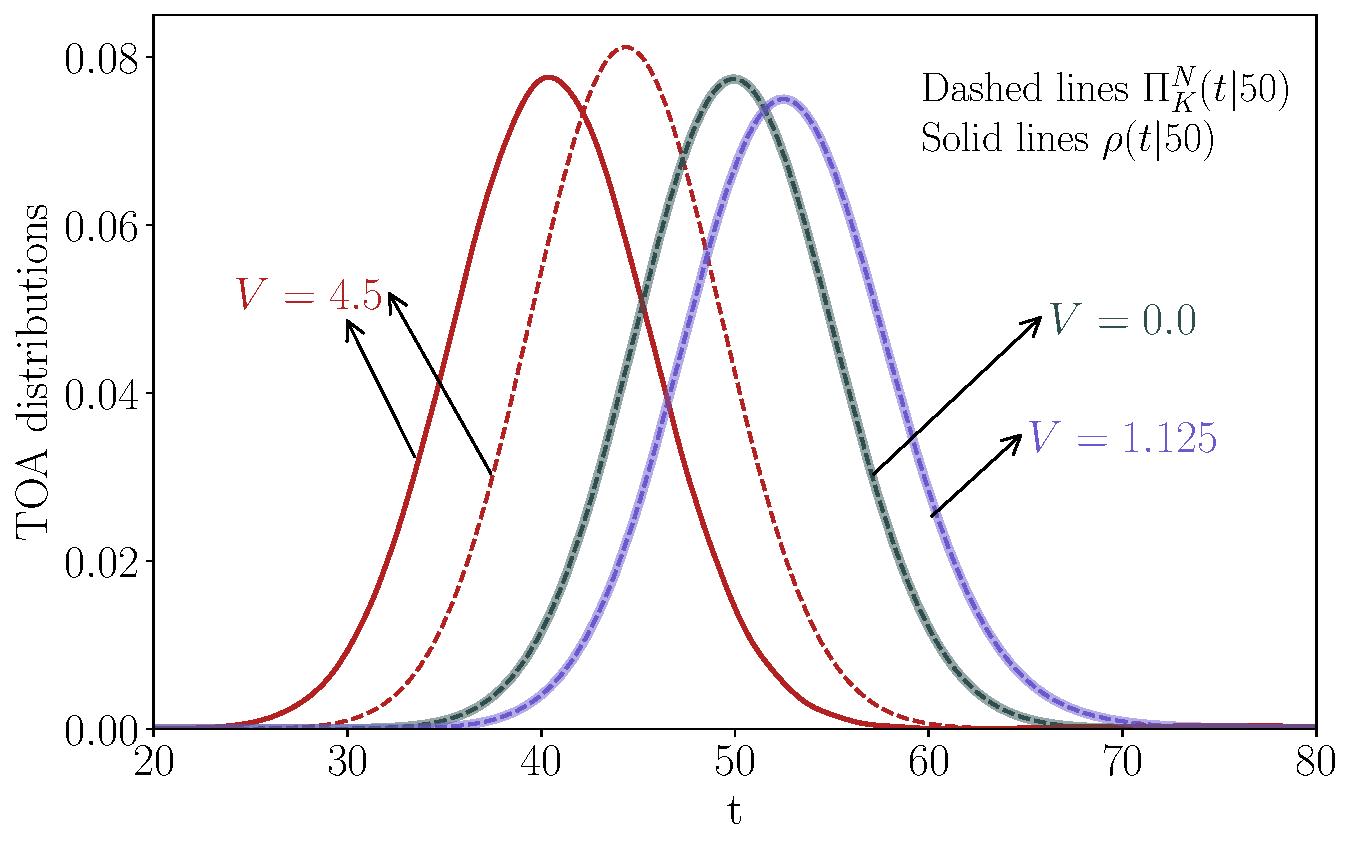
\includegraphics[width=14cm]{anexos/paper.pdf}
    \caption{Distribuições de probabilidade para o tempo de chegada das partículas transmitidas em $x=50$. O pacote de onda inicial, $\psi(x,t_i)$, possui $P_0=2$, $\delta=10$, $x_0=-50$ e $m=1$. A largura da barreira é $L = 10$. A linha contínua (trecejada) ilustra a previsão de $\rho(t|x)$ ($\Pi_K^N(t|x)$). Note que essas distribuições discordam no regime de tunelamento.}
    \label{fig:paper}
\end{figure}


Nós plotamos a distribuição de probabilidade do TOA na figura acima usando os mesmos parâmetros físicos da Ref.~\cite{Leon}. Essa referência obtém a Eq.~(\ref{KijoG}) transformando canonicamente o TOA da partícula livre. No gráfico, a largura da barreira é $L=10$, o detector está em $x=50$, e os parâmetros do pacote de onda inicial~(\ref{initialX}) são $x_i=-50$, $P_0=2$, $\delta= 10$ e $m=1$. As curvas sólidas e tracejadas mostram a distribuição do TOA em $x=50$ usando as Eqs.~(\ref{SolTBarrier}) e~(\ref{KijoG}), respectivamente, para $V_0=0 $, $V_0=1.125$ e $V_0=4.5$. Este último representa o regime de tunelamento. Observe que o TOA clássico de uma partícula livre com velocidade $P_0/m=2$ é $50$, já que o comprimento total do caminho da partícula é $100 $ unidades.



Ao inspecionar a Fig.~\ref{fig:paper} primeiro observamos que em comparação com a situação de transmissão livre, $V_0=0$, tanto as curvas sólidas quanto as tracejadas ilustram um atraso do TOA para $V_0<E_0=P_0^2/(2m)$ e avanço para $V_0>E_0$. Além disso, embora as expressões~(\ref{SolTBarrier}) e~(\ref{KijoG}) sejam matematicamente diferentes, elas concordam muito bem para $V_0<E_0$. No entanto, no regime de tunelamento, vemos que a Eq.~(\ref{SolTBarrier}) antecipa o tempo de chegada em relação à previsão da Eq.~(\ref{KijoG}). Essa discordância mostra que se as relações ${\tilde \phi}^+(P)={\tilde \psi}(P)$ e ${\tilde \phi}^+_T(P)={\tilde \psi }_{T}(P)$ estão corretos, a extensão STS deve ser reformulada de alguma forma. No entanto, se ${\tilde \phi}^+(P) \neq {\tilde \psi}(P)$ e/ou ${\tilde \phi}^+_T(P) \neq {\tilde \psi }_{T}(P)$, a solução~(\ref{SolTBarrier}) ainda pode estar correta.



Voltando ao que discutimos anteriormente, o conflito acima pode vir do fato de que $\phi^+(t|x)$ e $\phi^-(t|x)$ são tratados independentemente na Eq. ~(\ref{SolTBarrier}). Observe que $\phi^+(t|x)$ e $\phi^-(t|x)$ são desacoplados tanto na equação de Schrodinger EC~(\ref{Schro2T}) quanto na distribuição de probabilidade temporal~(\ref {rhoT}). Esse tratamento negligencia, por exemplo, a interferência entre momentos positivos e negativos. Essa independência também ocorre na distribuição Kijowski e foi originalmente criticada por Leavens \cite{LeavensR}. Vale ressaltar que usando a técnica de normalização de operador mencionada no Cap.~\ref{chap:cap2} para um potencial absorvedor fraco e estreito (definindo a região iluminada), Ref.~\cite{Heger2} generaliza a distribuição Kijowski levando em conta a interferência entre momentos positivos e negativos. Com essa discussão em mente, mudanças fisicamente plausíveis na extensão STS para acoplar as funções de onda EC de momentos positivos e negativos estão sendo investigadas para um próximo trabalho. 





